%-----------------------------------------------------------------------------
%
%               Template for sigplanconf LaTeX Class
%
% Name:         sigplanconf-template.tex
%
% Purpose:      A template for sigplanconf.cls, which is a LaTeX 2e class
%               file for SIGPLAN conference proceedings.
%
% Guide:        Refer to "Author's Guide to the ACM SIGPLAN Class,"
%               sigplanconf-guide.pdf
%
% Author:       Paul C. Anagnostopoulos
%               Windfall Software
%               978 371-2316
%               paul@windfall.com
%
% Created:      15 February 2005
%
%-----------------------------------------------------------------------------

\documentclass[preprint]{sigplanconf}

% The following \documentclass options may be useful:

% preprint      Remove this option only once the paper is in final form.
% 10pt          To set in 10-point type instead of 9-point.
% 11pt          To set in 11-point type instead of 9-point.
% numbers       To obtain numeric citation style instead of author/year.

\usepackage{pseudocode}
\usepackage{amsmath}
\usepackage{graphicx}
\usepackage{amsthm}
\usepackage{amsfonts}

\newcommand{\cL}{{\cal L}}

\newcommand{\func}[1]{{\sc #1}}
\newcommand{\farray}{\text{sequence}}
\newcommand{\tfunc}[1]{{\text{\func{#1}}}}
\newcommand{\val}{\func{val}}
\newcommand{\tval}{\text{\func{val}}}
\newcommand{\abs}{\func{abs}}
\newcommand{\new}{\func{new}}
\newcommand{\cost}{\func{cost}}
\newcommand{\tabulate}{\func{tabulate}}
\newcommand{\get}{\func{get}}
\newcommand{\set}{\func{set}}
\newcommand{\push}{\func{push}}
\newcommand{\size}{\func{size}}
\newcommand{\tget}{\text{\get}}
\newcommand{\tset}{\text{\set}}
\newcommand{\tpush}{\text{\push}}
\newcommand{\tsize}{\text{\size}}
\newcommand{\tnew}{\text{\new}}
\newcommand{\ttab}{\text{\tabulate}}
\newcommand{\MutableArray}{\text{MutableArray }}
\newcommand{\ArrayData}{\text{ArrayData }}
\newcommand{\Array}{\text{Array }}
\newcommand{\intref}{\text{int ref }}

\begin{document}

\special{papersize=8.5in,11in}
\setlength{\pdfpageheight}{\paperheight}
\setlength{\pdfpagewidth}{\paperwidth}

\conferenceinfo{CONF 'yy}{Month d--d, 20yy, City, ST, Country}
\copyrightyear{20yy}
\copyrightdata{978-1-nnnn-nnnn-n/yy/mm}
\copyrightdoi{nnnnnnn.nnnnnnn}

% Uncomment the publication rights you want to use.
%\publicationrights{transferred}
%\publicationrights{licensed}     % this is the default
%\publicationrights{author-pays}

% \titlebanner{banner above paper title}        % These are ignored unless
% \preprintfooter{short description of paper}   % 'preprint' option specified.

\title{Parallel Functional Arrays}

% \authorinfo{}{}{\\[-3.0ex]}
\authorinfo{Ananya Kumar}
           {Carnegie Mellon University}
           {ananyak@andrew.cmu.edu\\[-5.0ex]}
\authorinfo{Guy E. Blelloch}
           {Carnegie Mellon University}
           {blelloch@cs.cmu.edu}
\authorinfo{Robert Harper}
           {Carnegie Mellon University}
           {rwh@cs.cmu.edu}
\maketitle

\newtheorem{theorem}{Theorem}[section]
\newtheorem{corollary}{Corollary}[theorem]
\newtheorem{lemma}[theorem]{Lemma}
\theoremstyle{definition}
\newtheorem{definition}{Definition}[section]

\begin{abstract}
The goal of our paper is to come up with functional arrays (sequences) that are as efficient as imperative arrays, can be used in parallel, and have well defined cost-semantics. Our approach is to consider arrays with functional value semantics but non functional cost semantics. Because the value semantics is functional, ``updating" an array returns a new array. We allow operations on ``older" arrays (called interior arrays) to be more expensive than operations on the ``most recent" arrays (called leaf arrays) . 

We embed sequences in a language that supports fork join parallelism. Because we support fork-join parallelism, the cost of programs is non-deterministic and depends on the order in which operations are interleaved. This is because the ordering of operations can affect whether a sequence is a leaf or interior. Consequently the concurrent costs of such programs are difficult to analyze. Our main result is the derivation of a deterministic evaluational dynamics which makes analyzing the costs much easier. Our theorems are not array-specific and can be applied to any data type with different costs for operating on interior and leaf versions.

We give a wait-free concurrent sequence implementation which requires constant work for accessing and updating leaf arrays and bounded work for operations on interior arrays. We sketch out our proof of correctness for the array implementation. The key advantages of our sequence approach compared to current approaches is that our implementation requires no changes to existing programming languages, supports nested parallelism, and has well defined cost semantics. At the same time, it allows for functional implementations of algorithms like depth-first search with the same asymptotic complexity as imperative implementations.
\end{abstract}

\category{D.3.1}{Programming Languages}{Formal Definitions and Theory}
\category{F.3.2}{Logics and Meanings of Programs}{Semantics of Programming Languages}

\keywords
cost semantics, concurrency, parallel, functional data structures, persistence, arrays

\section{Introduction}
\label{sec:intro}

Supporting sequences (arrays) with efficient (constant time) random
access updates has been a persistent problem in functional languages
(pun intended).  It is easy to implement such sequences with constant
time random access reads (using arrays stored as contiguous memory),
or to implement with logarithmic time reads and updates using balanced
trees, but getting both in constant time cannot be done without some
form of extension.
%~\cite{Pippenger97}.  
This means that algorithms
for many fundamental problems are a logarithmic factor slower in
functional languages than in imperative languages.  This includes
algorithms for basic problems such as generating a random permutation,
and for many important graph problems (e.g.,
shortest-unweighted-paths, connected components, biconnected
components, topological sort, and cycle detection).  Simple algorithms
for these problems take linear time in the imperative setting, but an
additional logarithmic factor in time in the functional setting, at
least without extensions.

A variety of approaches have been suggested to alleviate this problem.
Many of the approaches are based on the observation that if there is
only a single reference to an array, it can be safely updated in
place.  The most common such approach is to use
monads~\cite{Moggi89,Wadler95}.  Monads can force code to be single
threaded and can thread mutable arrays (or other mutable
state) implicitly so the only reference to them is the current one.
Haskell supplies the ST monad for this purpose.  King and Launchbery,
for example, use STMonads with an array to implement depth first (DFS)
search in linear work~\cite{KL95}.  Guzman and Hudak's single-threaded
lambda calculus also uses the idea of single threading the
computation~\cite{GH90}, and motivate the approach based on allowing
for fast array updates.  The problem with using these approaches is
that it is basically implementing a second imperative language within
a functional language.  Using monads means using a new syntax not just
for the operations themselves but for everything the operations are
embedded in.  Indeed King and Launchbery have to write completely
different code for DFS, even though it is only for efficiency and not
correctness (it is trivial to implement DFS in $O(m \log n)$ time
purely functionally).  Monads also do not allow keeping persistent
versions of structures, exactly because the state can be changed.
More importantly, however, it forces the program itself to be single
threaded, inhibiting parallelism.

A second approach is to use a type system that enforces the
single-threadedness of individual arrays rather than the program as a
whole.  This can be done with linear types~\cite{Girard87,Wadler90},
which can be used to ensure that references are not duplicated.  This
is more flexible than monads, since it allows the threading of the
data to be distinct from the threading of the program.  However, such
type systems are not available in most languages, and they can be hard
to reason about.

A third approach is to support fully functional arrays in a general
functional language, and to check in the program if they happen to be
used in a single threaded manner.  This can be done, for example, by
using reference counting~\cite{HB85,Hudak86}.  The idea is to keep
track of how many references there are to an array and update inplace
if there is only one.  Hudak describes techniques to statically
analyze code to determine that at certain points in the code a count
must be one, and therefore it is safe to replace an update with an
inplace update.  The problem with this approach is that the efficiency
of the code depends heavily on the effectiveness of the compiler and
the specific way the code is written, and it can therefore be hard for
the user to reason about efficiency.

The last approach is to fully support functional arrays, even with
sharing, but more efficiently than as a simple array or tree.  This is
sometimes referred to as version tree arrays~\cite{AHN88} or fully
persistent arrays~\cite{DSST89}.  The idea is to maintain a version
tree for an array (or more generally other data types), such that any
node of the tree can be updated to create a new leaf below it with the
modified value, without effecting the value of other nodes.  Dietz
showed that arrays can be maintained fully persistently using
$O(\log\log n)$ time per operation (read or write).  Holmstrom, Hughes
and others (see \cite{AHN88}) suggested storing a version tree by
keeping the full array at the root, and a each node represents an
update.  Chuang's approach ~\cite{chuang} supports $O(1)$ accesses and
insertions to the most recent version of arrays, however accessing old
versions of the array takes $O(n)$ work which is often impractical.
O'Neill and Warren~\cite{oneill} describe various improvements.
The problem with these approaches is that they can be very complicated,
and only efficient in certain cases.   Furthermore it can be hard to
reason about the performance.

None of the existing approaches support concurrent operations on
arrays.  O' Neill suggests (in passing) having a lock for each element
of the array. However, when many threads contend for the same element,
this would serialize accesses and make accesses not
$O(1)$. Additionally, per-element locks add significant memory
overhead.  
% Separation logic ~\cite{reynolds} could be used to
% parallelize divide and conquer algorithms on arrays however they would
% severely restrict the way functional arrays can be used.

\subsection*{Our Approach}

In this paper we present an approach for efficiently supporting
functional arrays.  It uses some ideas from the previous approaches
but unlike the previous approaches it supplies a well
defined cost semantics, and supports parallelism, and without language
extensions.  More specifically the approach has the
following important features.
\begin{enumerate}
\item It has fully functional value semantics (dynamic
  semantics)---i.e., when not considering costs, arrays act no
  differently than purely functional arrays.
\item It requires no changes in existing languages and no special
  types, syntactic extensions, etc.  Programs can be efficient---i.e.,
  constant time reads and writes---when using a completely standard
  functional programming style.
\item The approach supports nested parallelism---arrays can be passed
  to parallel calls and safely updated and read, again with a purely
  functional semantics.
\item We supply a well defined cost semantics, which can be used to
  formally analyze the cost of any program.  The semantics captures
  both sequential and parallel costs.
\item We describe a cost-bounded implementation which maps costs in the
  model to costs on either a sequential or parallel RAM (PRAM).
\item
Although accessing old versions of an array is more expensive than
accessing new versions (as defined in the cost semantics), reading old
versions never costs more than $O(\log n)$ work.
\end{enumerate}
We have implemented the approach and in this paper present some
performance numbers.

Although our value semantics are purely functional (and compositional)
our cost semantics are not---they require passing a store and modeling
costs based on the order the store is threaded.  The reader might
object to this non-functional nature of the cost semantics, but we
note that non-functional costs are also requires in call-by-need
(lazy) languages, which supply a functional value semantics but an
imperative cost semantics.  In fact from the value point of view,
call-by-need is no different from call-by-name, and it is only when
considering costs that they differ.  The cost semantics of
call-by-need~\cite{AMOFW95} is completely non-functional
(non-compositional).  Furthermore it is likely significantly more
complicated to reason about than the cost semantics we present in this
paper.

\begin{figure}[!ht]
\centering 
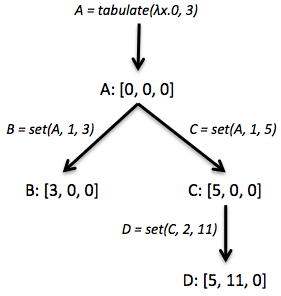
\includegraphics[scale=0.45]{leaf_interior_intro}
\nocaptionrule \caption{Example usage of functional arrays}
\label{fig:leaf_interior_intro}
\end{figure}

In this paper we consider arrays with three functions: \tabulate{},
\get{} (read), and \set{} (write).  As usual, \tabulate{}$(f,n)$
creates a new array of length $n$ by applying the function $f$ to
$[0, \ldots, n-1]$, \get$(A,i)$ returns the $i^{th}$ element of $A$, and
\set$(A,i,v)$ sets the $i^{th}$ element of $A$ to $v$ returning a
``new'' array (in the following discussion $n$ refers to the length of
an array).  Figure~\ref{fig:leaf_interior_intro} gives an example.  As
in previous work~\cite{AHN88} the history of an array after it is
created with \tabulate{} can be viewed as a version tree.  A version
tree has interior nodes and leaves.  In the figure, after all
functions are applied, arrays $A$ and $C$ are \emph{interior nodes},
and arrays $B$ and $D$ are \emph{leaves} of the version tree.  In our
cost semantics applying \get{} and \set{} to arrays at the leafs takes
constant work, but applying them to interior nodes is more expensive.
We define a cost semantics that identifies whether an array is a leaf
or interior node and charges for the cost of \get{} and \set{}
appropriately.  This requires threading a store that maps labels
(corresponding to each array) to indicate whether the array is a leaf
or interior.

Since we are also interested in parallelism, we include fork-join
parallelism in our language and semantics.    Our cost semantics then
models the cost of arrays when used in parallel.  This is non-trivial
since parallel tasks can read and update an array in parallel.
To deal with this, we compute the work of each forked task separately,
and then charge additional work at the join point if an array is used
in both forks.

To implement our functional arrays, we maintain at each leaf of the
version tree an array of the most recent values.  We also keep with
each location a change-log that keeps track of values at interior
nodes of the version tree.  Applying \get{} to a leaf only requires a
lookup in the array.  Applying \set{} to a leaf only requires updating
the array, and adding an element to the change log for the old
version.  Applying \get{} to an interior nodes requires a binary
search on the change log, which can be bounded by $O(\log n)$ time.
To ensure that change logs do not get too large, whenever the total
size across all change logs reaches $n$, the array is copied.   This
requires $O(n)$ time, but can be amortized against the updates.
Applying \set{} to an interior node requires creating a new array,
and copying values to it.   This requires $O(n)$ time.    

We give a wait-free concurrent implementation that uses careful
synchronization. We prove linearizability of the implementation and
use that to prove that our arrays work correctly when used
concurrently. Finally, we give a provable implementation for our cost
dynamics.


\section{Language}
\label{sec:dynamics}

The notation we use for our language and dynamics is from ~\cite{pfpl2}.

We use a standard applicative-order, call by value source language defined as follows:
$$e = x \; | \; c  \; | \; \lambda (x,y).e \; 
| \; e_1 e_2 \; 
| \; (e_1, e_2) \; 
| \; (e_1~||~e_2) \; 
| \; \text{if } e_1 \; e_2 \; e_3$$

The constants $c$ contains the usual arithmetic types, such as the
natural numbers and numerical functions. The expression $(e_1||e_2)$
indicates that the two expressions can run in parallel, returning a
pair $(v_1, v_2)$ when both expressions are fully evaluated, while
$(e_1,e_2)$ generates a pair sequentially.  Sequential and parallel
pairs only differ in the cost dynamics---the value dynamics are
identical. Our language can be augmented to add support for recursion using \func{letrec} or a fixed point combinator.

\begin{definition}
The terminal (fully evaluated) values are lambda expressions, constants,
and pairs of terminal values, and are denoted by the judgement \func{val}.
\end{definition}

Our language also contains functions to work with sequences. \new{}$(n,v)$ evaluates to a sequence of size $n$ with the value $v$ at each index. \get{}$(A, i)$ evaluates to the $i^{\text{th}}$ element of sequence $A$. \set{}$(A, i, v)$ evaluates to a new sequence where the $i^{\text{th}}$ element of $A$ is substituted with $v$.


\section{Structural Dynamics}
\label{sec:structural}

Our goal is to bound the runtime cost of evaluating a program (in our language) on a $p$ processor machine. For this purpose, we define two separate structural (small step) cost dynamics for our language: the \emph{idealized parallel dynamics} and the \emph{interleaved dynamics}.

The parallel dynamics defines the parallel \emph{span} (or depth) of a
computation, which is intuitively the number of parallel steps
given an unbounded number of processors. It is a pure dynamics
and allows all parallel expressions to proceed on the same step.

The interleaved dynamics defines the total \emph{work} performed by a
computation, which can be thought of as the number of instructions
used by the computation (within constant factors). The dynamics is
not pure, requiring a store to keep track whether each sequence is a leaf or interior, so that different costs can be charged for \get{} and \set{} in the two cases.  To account for parallelism, the dynamics allows for non-deterministic interleaving of steps on parallel expressions.  In conjunction with the impure cost for \get{} and \set{}, this means the overall work is non-deterministic. In Section~\ref{sec:evaluational} we give a deterministic cost dynamics and
show that it provides an upper bound on the work over all possible
interleavings.

The two dynamics are useful together because we can bound the
runtime on any fixed number of processors based on the work and span.

\subsection{Idealized Parallel Dynamics}

The idealized parallel dynamics captures the evaluation steps taken on a
machine with an unbounded number of processors and
is given by the following judgement, where $e$ is the expression and
$e'$ is the resulting expression:
$$e \to_{par} e'$$

Let $\overline{\text{\get{}}}(A, i)$ denote $A[i]$, $\overline{\text{\set{}}}(A, (i,v))$ denote $A[i \mapsto v]$ (which denotes the sequence obtained if the value at index $i$ of $A$ is replaced with $v$), and $\overline{\text{\new{}}}((n,v))$ denote a sequence of size $n$ with the value $v$ at each index. Intuitively, $\overline{\text{\get{}}}$, $\overline{\text{\set{}}}$, and $\overline{\text{\new{}}}$ represent abstract versions of \get{}, \set{}, and \new{}.

We show the rules for get and fork-join in Figure \ref{fig:parallel-dynamics}. As usual, the judgement \func{val} describes terminal values. Notice that in fork-join, both sides of the fork-join take a step at the same time if possible. The rules for \set{} and \new{} are similar to the rules for \get{}, and the rules for function application and if-then are as in a standard applicative order functional programming language. 

\begin{figure}
$$\frac{A, a \; \text{val}}{\tget{}(A, a) \to_{par} \overline{\mbox{\get{}}}(A, a)} \text{ (get-eval)}$$
$$\frac{e_1 \to_{par} e_1' \;\;\; e_2 \to_{par} e_2'}{e_1 || e_2 \to_{par} e_1' || e_2'} \text{ (fork)}$$
$$\frac{v_1 \; \text{val} \;\;\; e_2 \to_{par} e_2'}{v_1 || e_2 \to_{par} v_1 || e_2'} \text{ (step-right)}$$
$$\frac{v_2 \; \text{val} \;\;\; e_1 \to_{par} e_1'}{e_1 || v_2 \to_{par} e_1' || v_2} \text{ (step-left)}$$
$$\frac{v_1, v_2 \text{ val}}{(v_1 || v_2) \to_{par} (v_1, v_2)} \text{ (join)}$$

\caption{Example rules in the parallel dynamics for our language.}
\label{fig:parallel-dynamics}
\end{figure}

The parallel structural dynamics, unlike the interleaved
structural dynamics, is deterministic.

\begin{definition}
A \emph{parallel transition sequence} $T$ is a sequence $(e_0, ..., e_n)$ with $e_i \to_{par} e_{i+1}$ for all $0 \leq i < n$. We say that $e_0 \to^n_{par} e_n$ or $e_0 \to^*_{par} e_n$.
\end{definition}

\begin{definition}
The \emph{span} of a parallel transition sequence $T$, denoted by $SP(T)$, is its length $n$.
\end{definition}

\subsection{Interleaved Cost Dynamics}

The interleaved dynamics is a concurrent dynamics and is given by the following judgement, where $\sigma$ is the
store, $e$ is the expression, $\sigma'$ is the resulting store, $e'$ is the
resulting expression after a step has been taken, and $w$ is the work.
$$\sigma, e \to \sigma', e', w$$

Sequence values are represented by the pair $(l, V)$ where $l$ is a
label into the store $\sigma$ and $V$ is a list of the elements in the sequence.  The store is a mapping from labels to either $+$ (indicating a leaf sequence)
or $-$ (indicating an interior sequence). Let $L(\sigma)$ denote the set of labels in the store $\sigma$.

Let $g_l(V)$ and $g_i(V)$ be the work of \get{} applied to $V$ if it
is a leaf or interior sequence, respectively, and $s_l(V)$ and $s_i(V)$
be the work of \set{} applied to $V$ if it is a leaf or interior
sequence.  Let $n(a)$ be the work of evaluating \new{}$(a)$.  We assume
that $g_l(V) \leq g_i(V)$ and $s_l(V) \leq s_i(V)$ (operating on leaf
sequences is cheaper that operating on interior sequences).

\begin{figure}
$$\frac{v_1, v_2 \; \text{val}}{\sigma, (\lambda (x,y).e)(v_1,v_2) \to \sigma, [v_1/x][v_2/y]e, 1} \text{ (func-app)}$$

$$\frac{}{\sigma, \text{if } \text{true} \; e_2 \; e_3 \to \sigma, e_2, 1} \text{ (if-true)}$$

$$\frac{}{\sigma, \text{if } \text{false} \; e_2 \; e_3 \to \sigma, e_3, 1}  \text{ (if-false)}$$

$$\frac{a \; \text{val} \;\;\; l \not\in L(\sigma)}{\sigma, \tnew{}(a) \to \sigma[l \mapsto +], \overline{\mbox{\new{}}}(a), n(a)} \text{ (new)}$$

$$\frac{A = (l, V) \;\;\; \sigma[l] = + \;\;\; a \text{ val}}{\sigma, \tget{}(A, a) \to \sigma, \overline{\mbox{\get{}}}(V,a), g_l(V)} \text{ (get-leaf)}$$

$$\frac{A = (l, V) \;\;\; \sigma[l] = -  \;\;\; a \text{ val}}{\sigma, \tget(A, a) \to \sigma, \overline{\mbox{\get{}}}(V,a), g_i(V)} \text{ (get-interior)}$$

$$\frac{A = (l, V) \;\;\; \sigma[l] = + \;\;\;  l' \not\in L(\sigma) \;\;\; a \text{ val}}{\begin{gathered}\sigma, \tset(A, a) \to \sigma[l \mapsto -, l' \mapsto +], \\ (l', \overline{\mbox{\set{}}}(V, a)), s_l(V)\end{gathered}} \text{ (set-leaf)}$$

$$\frac{A = (l, V) \;\;\; \sigma[l] = - \;\;\;  l' \not\in L(\sigma) \;\;\; a \text{ val}}{\begin{gathered}\sigma, \tset(A, a) \to \sigma[l' \mapsto +], \\ (l', \overline{\mbox{\set{}}}(V,a)), s_i(V)\end{gathered}} \text{ (set-interior)}$$

$$\frac{\sigma, e_1 \to \sigma', e_1', w}{\sigma, e_1 || e_2 \to \sigma', e_1' || e_2, w} \text{ (step-left)}$$
$$\frac{\sigma, e_2 \to \sigma', e_2', w}{\sigma, e_1 || e_2 \to \sigma', e_1 || e_2', w} \text{ (step-right)}$$
$$\frac{v_1, v_2 \text{ val}}{\sigma, (v_1 || v_2) \to \sigma, (v_1, v_2), 1} \text{ (join)}$$

\caption{The interleaved dynamics for our language.  We omit
  rules that involve stepping the arguments to \get{}, \set{}, \new{},
  and other language constructs.}
\label{fig:interleaved}
\end{figure}

The dynamics is given in figure~\ref{fig:interleaved}.  Note that
\set$(A,a)$ where $A = (l,V)$ and $\sigma[l] = +$ creates a new label and
value, extends the store to indicate the new value is a leaf, and
updates the store at $l$ to indicate that $A$ is now interior.  This
is the impure aspect of the cost dynamics since there can be other
references to $l$.  Also note that the work for for \get{} and \set{}
depends on whether the sequence is a leaf or interior.

The rules for fork-join are non-deterministic---either side of the
fork can take a step.  This allows for arbitrary interleaving of
instructions on different sides of a fork-join.  After both sides of a
fork-join are fully evaluated the parallel pair is converted to a regular pair.

\begin{definition}
A \emph{transition sequence} $T$ is a sequence of states $[(\sigma_0, e_0),
..., (\sigma_n, e_n)]$ and per-step work $[w_1, ..., w_n]$ s.t. for all $0 \leq i < n$, $\sigma_i, e_i \to \sigma_{i+1}, e_{i+1}, w_{i+1}$ . We say that $T$ takes $\sigma_0, e_0$ to $\sigma_n, e_n$ and has length $n$ and denote this by $\sigma_0, e_0 \to^n \sigma_n, e_n$.
\end{definition}

\begin{definition}
We say that $T$ is \emph{maximal} if there does not exist $\sigma', e', w'$ s.t. $\sigma_n, e_n \to \sigma', e', w'$.
\end{definition}

\begin{definition}
A \emph{transition subsequence} $T_{i, j}$ of $T$ is given by the
sequence of states $[(\sigma_i, e_i), ..., (\sigma_j, e_j)]$ and per-step work
$[w_{i+1}, ..., w_j]$. Note that $T = T_{0,n}$.   
\end{definition}

\begin{definition}
The \emph{work of a transition sequence} $T$ is given by:
$$W(T) = \sum_{i=1}^n w_i$$
\end{definition}

Different transition sequences starting and ending at the same states
may have different work.  In particular, a sequence can be used
concurrently by multiple parallel expressions and the work could
depend on the order in which the instructions are interleaved.
Figure~\ref{fig:fork_join_intuition} shows 3 ways a leaf sequence $A$
might be used.  In particular, one side of the fork might call \get{}
on $A$ while the other side calls \set{} (see the center panel). Calls
to \get{} on the left branch would have work $g_l(A)$ if and only if
they execute before the call to \set{} on the right branch, otherwise
they would have work $g_i(A)$.

\begin{figure}[!ht]
\centering
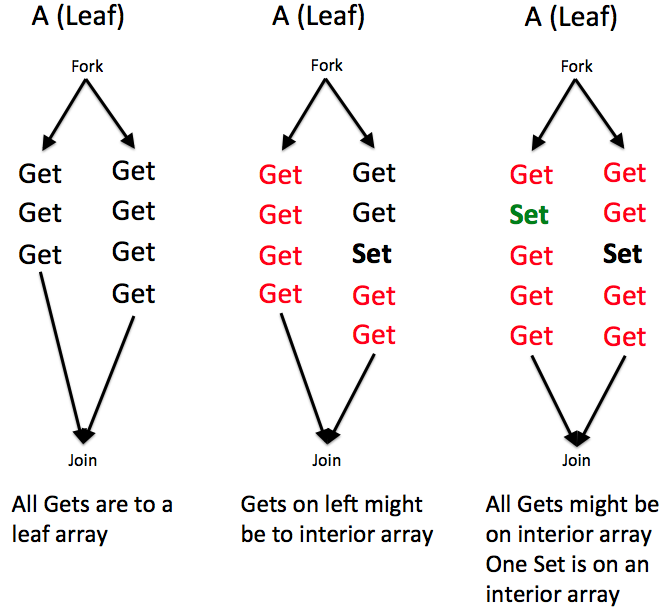
\includegraphics[scale=0.3]{fork_join_intuition}
\nocaptionrule \caption{Different ways a sequence might be used in a fork join}
\label{fig:fork_join_intuition}
\end{figure}

We cannot make any assumptions about how the instructions in different
branches of a fork are interleaved, so we need to capture the worst
case work over all possible interleavings.

\begin{definition}
Let $w$ be the max of $W(T)$ over all transition sequences starting at $\sigma_0, e_0$. If $W(T)$ is unbounded then $w = \infty$. $w$ is the \emph{work of evaluating} $\sigma_0, e_0$. 
\end{definition}

\subsection{Machine Costs}

We now consider the cost of evaluating an expression on a shared
memory machine with $P$ processors.  We assume that
within a constant factor, the cost functions $g_l(V)$,
$g_i(V)$, $s_l(V)$, $s_i(V)$, and $n(a)$ are upper bounds on the
number of instructions needed by the implementation for each of the
corresponding functions.  In this case we say the cost functions have
valid work bounds. In Section~\ref{sec:implementations} we describe an implementation and prove work bounds for sequences. 

\new{}, \get{} and \set{} can each have parallelism in their implementation, so in addition to the work we need to know the span for these functions (the number of time steps on an unbounded number of processors). Here we assume the span for \new{}, \get{}, and \set{} is bounded by some $f(P)$ where $P$ is the number of processors used.   

Using the greedy scheduling theorem ~\cite{BlumofeLeiserson} or Brent's
theorem~\cite{brent} knowing the total work and total span (number of
steps on an unbounded number of processors) is sufficient to bound the
time on any finite number of processors. We assume that standard instructions such as reading and writing to memory, arithmetic operations, etc. take constant time (and work). This leads to the following theorem.

\begin{theorem}
\label{thm:brent}
Given cost functions with valid work bounds each with maximum span
$f(p)$, then for any expression $e$ with a constant number of
variable names if $w$ is the work of evaluating $\sigma, e$, and $S$ is the span for the (unique) maximal transition sequence starting at $e$, then $e$ can be evaluated using any greedy schedule on a $P$ processor machine in time
\[ T \leq c \left(\frac{w}{P} + S f(P)\right)\]
for some constant $c$ that is independent of the expression $e$.
\end{theorem}
\begin{proof} (outline).  This follows from the greedy scheduling theorem and previous work on bounded cost implementations. Bounding the number of variables is needed to bound the cost of evaluating each step of the program itself ~\cite{BG95}. It avoids issues of non-constant cost for looking up the values of variables in environments.
\end{proof}


\section{Evaluational Cost Dynamics}
\label{sec:evaluational}

The evaluational (big-step) cost dynamics gives an easy, deterministic way to compute the cost of a program without having to reason about multiple interleavings. In this section, we give the rules for the evaluational dynamics. In section~\ref{sec:costproof}, we prove that the costs in the evaluational dynamics are a tight upper bound for the costs in the structural dynamics. Our results can be easily extended for data types besides sequences (like unordered sets) even if there are multiple varieties of \get{} and \set{} functions.

To handle the non-determinism in fork-join, we first compute the worst-case cost of each fork separately. Then for sequences that are used in both forks, we add additional work at the join point. To compute the additional work at the join point, we keep track of the number of \get{}s to leaf values on each side of the fork. If the value was \set{} on the other side of the fork, then the \set{} might have happened before the \get{}s, so we need to charge additional work for the \get{}s.

Our evaluational dynamics is defined by the following judgement, where $\delta$ is the store, $e$ is the expression, $\delta'$ is the new store, $v$ is the value that $e$ evaluates to, $w$ is the work, and $s$ is the span.
$$\delta, e \boldsymbol\Downarrow \delta', v, w, s$$

As in the previous section, sequences are represented by $(l, V)$ where $l$ is a label into the store $\delta$ and $V$ is a list of the elements in the sequence. The store is a mapping from labels to $(+/-, c)$, where $c$ represents the number of leaf \get{}s on the value indexed by the label. $L(\delta)$ denotes the set of labels in the store $\delta$.

The rules in the evaluational dynamics are given in figure \ref{fig:evaluational-dynamics}. Note that \get{} costs $g_l(V)$ instead of $g_i(V)$ on a leaf value $V$ but we increment the counter of leaf \get{}s in the store. 

\begin{figure}[!ht]
$$\frac{}{\delta, c \Downarrow \delta, c, 1, 1} \text{ (constants)}$$

$$\frac{\begin{gathered}\delta, e_1 \Downarrow \delta', \lambda (x,y) . e, w_1 , s_1 \;\;\; \delta', e_2 \Downarrow \delta'',(v_1, v_2), w_2 , s_2 \;\;\; \\ \delta'', [v_1/x][v_2/y]e \Downarrow \delta''', v', w_3 , s_3\end{gathered}}{\delta, e_1 \; e_2 \Downarrow \delta''', v', 1+w_1+w_2+w_3, 1+s_1+s_2+s_3} \text{ (func-app)}$$

$$\frac{\delta, e_1 \Downarrow \delta', true, w_1, s_1 \;\;\, \delta', e_2 \Downarrow \delta'', v, w_2, s_2}{\delta, \text{if } e_1 \; e_2 \; e_3 \Downarrow \delta'', v, 1+w_1+w_2, 1+s_1+s_2} \text{ (if-true)}$$

$$\frac{\delta, e_1 \Downarrow \delta', false, w_1, s_1 \;\;\; \delta', e_3 \Downarrow \delta'', v, w_2, s_2}{\delta, \text{if } e_1 \; e_2 \; e_3 \Downarrow \delta'', v, 1+w_1+w_2, 1+s_1+s_2} \text{ (if-false)}$$

$$\frac{\delta, e \Downarrow \delta', a, w, s \;\;\; l \not\in L(\delta')}{\begin{gathered}\delta, \tnew{}(e) \Downarrow \delta'[l \mapsto (+,0)], \overline{\mbox{\new{}}}(a), w + n(a), s+1\end{gathered}} \text{ (new)}$$

$$\frac{A = (l,V) \;\;\; a \text{ val} \;\;\; \delta[l \mapsto (+, c)] \;\;\; l' \not\in L(\delta)}{\begin{gathered}\delta, \tset(A, a) \Downarrow \delta[l \mapsto (-, c), l' \mapsto (+, 0)], \\ (l', \overline{\mbox{\set{}}}(V, a)), s_l(V), 1\end{gathered}} \text{  (set-leaf)}$$

$$\frac{A = (l,V) \;\;\; a \text{ val} \;\;\; \delta[l \mapsto (-, c)] \;\;\;  l' \not\in L(\delta)}{\begin{gathered}\delta, \tset(A, a) \Downarrow \delta[l' \mapsto (+, 0)], \\ (l', \overline{\mbox{\set{}}}(V, a)), s_i(V), 1\end{gathered}} \text{  (set-int)}$$

$$\frac{\begin{gathered}\delta; e_1 \Downarrow \delta_1, A, w_1, s_1 \;\;\; \delta_1, e_2 \Downarrow \delta_2, a, w_2, s_2 \;\;\; \\ \delta_2, \tset(A, a) \Downarrow \delta', A', w', s' \end{gathered}}{\delta, \tset(e_1, e_2) \Downarrow \delta', A', w_1+w_2+w', s_1+s_2+s'} \text{ (set-eval)}$$  

$$\frac{A = (l,V) \;\;\; a \text{ val} \;\;\; \delta[l \mapsto (+, c)]}{\begin{gathered}\delta, \tget{}(A, a) \Downarrow \delta[l \mapsto (+, c+1)], \\ \overline{\mbox{\get{}}}(V, a), g_l(V), 1\end{gathered}} \text{  (get-leaf)}$$

$$\frac{A = (l,V) \;\;\; a \text{ val} \;\;\; \delta[l \mapsto (-, c)]}{\delta, \tget{}(A, a) \Downarrow \delta, \overline{\mbox{\get{}}}(V, a), g_i(V), 1} \text{  (get-interior)}$$

$$\frac{\begin{gathered}\delta, e_1 \Downarrow \delta_1, A, w_1, s_1 \;\;\; \delta_1, e_2 \Downarrow \delta_2, a, w_2, s_2 \;\;\; \\ \delta_2, \tget{}(A, a) \Downarrow \delta', v', w', s' \end{gathered}}{\delta, \tget(e_1, e_2) \Downarrow \delta', v', w_1 + w_2 + w', s_1 + s_2 + s'}\text{ (get-eval)}$$

$$\frac{\begin{gathered}\delta, e_L \Downarrow \delta_L, v_L, w_L, s_L \;\;\; \delta, e_R \Downarrow \delta_R, v_R, w_R, s_R \;\;\; \\ (L(\delta_L) \setminus L(\delta)) \cap (L(\delta_R) \setminus L(\delta)) = \emptyset\end{gathered}}{\delta, (e_L || e_R) \Downarrow \delta', (v_L, v_R), 1 + w_L + w_R + w', 1 + \max(s_L, s_R)} \text{  (fj)}$$

\caption{Rules for the evaluational dynamics. $w'$ and $\delta'$ in the fork-join rule are defined in the paper.}
\label{fig:evaluational-dynamics}
\end{figure}

The fork-join rule is the most interesting and requires a few definitions. Suppose we have expression $(e_L || e_R)$ with
\[ \delta, e_L \Downarrow \delta_L, v_L, w_L, s_L \]
\[ \delta, e_R \Downarrow \delta_R, v_R, w_R, s_R \]

Further, suppose that $(L(\delta_L) \setminus L(\delta)) \cap (L(\delta_R) \setminus L(\delta)) = \emptyset$ (the new labels produced on both sides of the fork-join do not conflict). Consider a sequence $A = (l, V)$ with $\delta[l] = (s,c)$, $\delta_L[l] = (s_L, c + c_L)$, $\delta_R[l] = (s_R, c + c_R)$. When multiplying two signs or multiplying a sign with an integer, consider $+$ to be 1 and $-$ to be 0. 

\func{Combine} describes how to combine store values on both sides of a fork-join. A sequence is a leaf iff it is a leaf on both sides of the fork-join. Leaf \get{}s on one side of the fork remain leaf \get{}s iff there were no calls to \set{} on the other side of the fork.
\begin{equation*}
  \begin{aligned}
   \text{\func{combine}}&((s, c), (s_L, c + c_L), (s_R, c + c_R))= \\
   &(s_L s_R, c + s_R c_L + s_L c_R)
  \end{aligned}
\end{equation*}
$$\delta' = \; (\delta_L / \delta) \; \cup \; (\delta_R / \delta) \; \cup \bigcup_{l \in L(\delta)} [l \mapsto \text{\func{combine}}(\delta[l], \delta_L[l], \delta_R[l])]$$
\func{Extrawork} gives the additional cost incurred if a sequence was modified on either side of a fork-join. If the value was interior before the fork-join, then all functions incurred their maximal cost and there is no additional cost. Otherwise, leaf \get{}s on one side of the fork are charged $g_i$ work iff the other side of the fork called \set{}. Additionally, if both sides of the fork called \set{}, then one of the \set{}s came first and has work $s_l$ and the subsequent \set{} has work $s_i$. We abuse notation so that $g_l, g_i, s_l, s_i$ directly take in a label $l$ instead of the corresponding sequence.
\begin{equation*}
  \begin{aligned}
  \text{\func{extra}}&\text{\func{work}}(l, (s, c), (s_L, c + c_L), (s_R, c + c_R)) = \\
  & ((\neg s_R) c_L  + (\neg s_L) c_R)(g_i(l)-g_l(l)) + \\
  & (\neg s_R) (\neg s_L) (s_i(l)-s_l(l))
 \end{aligned}
\end{equation*}
$$w' = \sum_{l \in L(\delta), \delta[l \mapsto (+, c)]} \text{\func{extrawork}}(l, \delta[l], \delta_L[l], \delta_R[l])$$
Then, the fork-join cost dynamics are:
$$\delta; (e_L || e_R) \Downarrow \delta'; (v_L || v_R); 1 + w_L + w_R + w'; 1 + \max(s_L, s_R)$$

\section{Cost Proofs}
\label{sec:costproof}

We show that the work computed by the evaluational dynamics is a tight upper bound for the work in the interleaved structural dynamics. Proofs for the span bounds are omitted because they are standard (the parallel structural dynamics is deterministic).

\begin{definition}
Consider a transition sequence $T$. We say that $S_i, e_i \to S_{i+1}, e_{i+1}, w_{i+1}$ is a \get{} on $l$ if the step involves evaluating the \get{} function on structure $(l, V)$. We say it is a \emph{cheap \get{}} on $l$ if $w_{i+1} = g_l(l)$. The number of cheap \get{}s on $l$ in $T$ is denoted by $SC_l(T)$.
\end{definition}

\begin{definition}
Unlike the store in the evaluational dynamics, the store in the structural dynamics only stores whether each structure is $+$ (leaf) or $-$ (interior). $sign(\delta)$ takes a store that maps $l \mapsto (s,c)$ and returns a store which maps $l \mapsto s$.
\end{definition}

\begin{definition}
Suppose that $\delta, e \Downarrow \delta', e', w', s'$. We define the number of cheap \get{}s in going from $\delta$ to $\delta'$ in the evaluational dynamics as follows. Suppose $l \mapsto (s', c') \in \delta'$. If $l \mapsto (s,c) \in \delta$ then $EC_l(\delta, \delta') = c' - c$ and if $l \not\in L(\delta)$ then $EC_l(\delta, \delta') = c'$. If $l \not\in L(\delta')$ then $EC_l(\delta, \delta') = 0$.
\end{definition}

\begin{definition}
A \emph{relabeling} of $L_1$ is a bijective function $R$ from label sets $L_1 \to L_2$. $R$ can be used to relabel stores and expressions. $R(\delta) = \{ R(l) \mapsto e \; | \; l \mapsto e \in \delta \wedge l \in L_1  \} \cup \{ l \mapsto e \; | \; l \mapsto e \in \delta \wedge l \not\in L_1  \}$. In other words, $R$ relabels some of the labels in $\delta$. Similarly, $R(e)$ returns an expression $e'$ where each occurrence of a label $l \in L_1$ in $e$ is substituted by $R(l)$.
\end{definition}

\begin{lemma}
\label{relabeling_lemma}
Suppose that there exists a derivation of length $m$ that $\delta, e \Downarrow \delta', e', w, s$. Let $R$ be an arbitrary labeling. Then there exists a derivation of length $m$ that $R(\delta), R(e) \Downarrow R(\delta'), R(e'), w, s$.
\end{lemma}

\begin{proof}
By applying the relabeling to each step of the derivation, and noting that all rules in the evaluational dynamics hold under relabelings.
\end{proof}

\begin{lemma}
\label{stateless_lemma}
If $S, e \to S', e', w$ and $U$ is a store s.t. for all $l \in e$, $l \in U$, then there exists $U', w'$ s.t. $U, e \to U', e', w'$
\end{lemma}

\begin{proof}
By casing on each rule in the structural dynamics, and noting that transitions of expressions never depend on the values in the store (the dynamics are purely functional).
\end{proof}

\begin{theorem}
\label{main_work_theorem}
Suppose that 
$$\delta, e_0 \Downarrow \delta_E, e_E, w_E, s_E$$

and consider arbitrary maximal transition sequence T taking 
$$S_0 = sign(\delta), e_0 \to^n S_n, e_n$$
å
The following hold:
\begin{enumerate}
\item For some relabeling $R$ of $L(\delta_E) \setminus L(\delta)$, $S_n = sign(R(\delta_E))$ and $e_n = R(e_E)$.
\item For all $l \in \delta_E$, $EC_l(\delta, \delta_E) \leq SC_{R(l)}(T)$.
\item The sum of work and cheap \get{}s is conserved: \begin{align*}
w_E + &\sum_{l \in L(\delta_E)} EC_l(\delta, \delta_E) (g_i(l)-g_l(l)) =\\
 &W(T) + \sum_{l \in L(\delta_E)} SC_{R(l)}(T) (g_i(R(l)) - g_l(R(l)))
 \end{align*}
\end{enumerate}
\end{theorem}

\begin{proof}
By induction on the length of the shortest derivation in the evaluation dynamics. We prove the theorem for 2 of the rules in the evaluation dynamics: get-leaf and fork-join. The other cases follow from a similar line of reasoning.
\\

\noindent \textbf{Case get-leaf}: Suppose $e_0 = \tget{}(e_L, e_R)$ and
$$\delta, e_L \Downarrow \delta_L, e_L', w_L$$
$$\delta_L, e_R \Downarrow \delta_R, e_R', w_R$$
$$\delta_R, \tget{}(e_L', e_R') \Downarrow \delta_E, e_E, g_l(l')$$
where $e_L' = (l', V)$ for some $V$, which gives us
$$\delta, \tget{}(e_L, e_R) \Downarrow \delta_E, e_E, w_E$$
with $w_E = w_L + w_R + g_l(l')$.

Note that the structural dynamics first step the left argument to \get{}, then the right argument, and finally evaluate the \get{}. So there exists $m$ such that $T_{0,m}$ involves stepping the left argument, $T_{m,n-1}$ involves stepping the right argument, and $T_{n-1,n}$ involves evaluating the \get{}.

\textbf{Part 1}: Suppose that in $T_{0,m}$, for $0 \leq i \leq m$, $e_i = get(e_{L,i}, e_R)$. Consider a new projected transition sequence $T_{0,m}'$ with states $[(S_0, e_{L,0}), ..., (S_m, e_{L,m})]$ and costs the same as $T_{0,m}$: $[w_1, ..., w_m]$. It is easy to verify that $T_{0,m}'$ is a valid transition sequence starting at $(S_0, e_{L,0})$ and is maximal. 

$S_0 = sign(\delta)$ and $e_{L,0} = e_L$ so we can apply the IH to $T_{0,m}'$. For some relabeling $R$ of labels in $L(\delta_L) / \delta$, $s_m = sign(R(\delta_L))$ and $e_{L,m} = R(e_L')$ $\Rightarrow$ $e_m' = (e_{L,m}, e_R) = (R(e_L'), e_R)$. WLOG suppose that $\delta_L$ was labeled such that the above hold (we can do this because of lemma \ref{relabeling_lemma}). Note that in subsequent parts of the proof, we omit creating the projected transition sequence and apply the IH directly to $T_{0,m}$ when needed.

Using similar logic on $T_{m,n-1}$ we get that for some relabeling of $\delta_R / \delta_L$, applying that relabeling to $\delta_R$ and $(e_L', e_R')$ gives us $e_{n-1} = (e_L', e_R')$ and $S_{n-1} = sign(\delta_R)$. WLOG suppose that $\delta_R$ was labeled so that the above holds.

By combining the relabelings of $\delta_L / \delta$ and $\delta_R / \delta_L$ and applying that to $(e_L', e_R')$ and $\delta_R$, we get that $e_{n-1} = get(e_L', e_R')$ and $S_{n-1} = sign(\delta_R)$. Note that get does not change the sign of any label in the store in either the structural or the evaluation dynamics, so $sign(\delta_E) = sign(\delta_R) = S_{n-1} = S_n$. Further, the structural and evaluational dynamics apply get in the same way, so $e_n = e_E$. Therefore the first part of this theorem holds. WLOG suppose that the stores and expressions were relabeled s.t. the first part holds.

\textbf{Part 2}: From lemma \ref{relabeling_lemma}, the length of the shortest derivation for the relabeled evaluational dynamics does not change, so we can apply the inductive hypothesis even after the relabeling. Applying the IH to $T_{0,m}$, for all $l \in \delta_L$, $EC_l(\delta, \delta_L) \leq SC_l(T_{0,m}') = SC_l(T_{0,m})$. If $l \in \delta_R$ but $l \not\in \delta_L$ then $EC_l(\delta, \delta_L) = SC_l(T_{0,m}) = 0$ (intuitively the label did not exist and so did not have any cheap gets), so in particular, for all $l \in \delta_R$, $EC_l(\delta, \delta_L) \leq SC_l(T_{0,m})$. Applying the IH to $T_{m,n-1}$ we get that for all $l \in \delta_R$, $EC_l(\delta_L, \delta_R) \leq SC(T_{m,n-1})$.

We note that $EC$ and $SC$ are additive, that is,
$$EC_l(\delta, \delta_R) = EC_l(\delta, \delta_L) + EC_l(\delta_L, \delta_R)$$
$$SC_l(T_{0,n-1}) = SC_l(T_{0,m}) + SC_l(T_{m,n-1})$$
This implies that for all $l \in \delta_R$, $EC_l(\delta, \delta_R) \leq SC_l(T_{0,n-1})$. 

Now, let $e_L' = (l',V)$ with $l' \in \delta_R$. Then, $EC_{l'}(\delta, \delta_E) = EC_{l'}(\delta, \delta_R) + 1$ and $SC_{l'}(T) = SC_{l'}(T_{0,n-1}) + 1$, so $EC_{l'}(\delta, \delta_E) \leq SC_{l'}(T)$. If $l \neq l'$ then $EC_{l}(\delta, \delta_E) = EC_{l}(\delta, \delta_R)$ and $SC_{l}(T) = SC_{l}(T_{0,n-1})$, so $EC_{l}(\delta, \delta_E) \leq SC_{l}(T)$. So the second part of the theorem holds.

\textbf{Part 3}: The third part of the theorem follows by similarly applying the IH on $T_{0,m}$ and $T_{m,n-1}$, and noting that $W(T) = W(T_{0,m}) + W(T_{m,n-1}) + g_l(l')$.
\\

\noindent \textbf{Case fork-join}: Suppose $e_0 = (e_L || e_R)$ and
$$\delta, e_L \Downarrow \delta_L, v_L, w_L$$
$$\delta, e_R \Downarrow \delta_R, v_R, w_R$$
which gives us
$$\delta, (e_L || e_R) \Downarrow \delta', (v_1 || v_2), w_L + w_R + w'$$
with $w'$ and $\delta'$ defined in terms of \func{extrawork} and \func{combine} as given in the evaluational dynamics.

In T, for all $0 \leq i \leq n$ let $e_i = (e^L_i || e^R_i)$. Let $I_L$ be the sequence of all $0 \leq i \leq n-1$ where transitioning from $e_i$ to $e_{i+1}$ involved stepping the left argument. Let $m$ be the length of $I_L$. Similarly define $I_R$ for the right argument, and let $k$ be the length of $I_R$.

Let $A$ be the sequence of $e^L$s corresponding the indices in $I_L$, and add $e^L_n$ at the end of $A$. Similarly, let $B$ be the sequence of $e^R$s corresponding the indices in $I_R$, adding $e^R_n$ at the end.

Let $S^L_0 = S_0 = sign(\delta)$. By inductively applying lemma \ref{stateless_lemma}, there exists $S^L_1, ... S^L_m$ s.t. $T_L = [(S^L_0, A_0), ..., (S^L_m, A_m)]$ is a transition sequence. $T_L$ is maximal, because if $A_m$ in $T_L$ can take a step then $e^L_n$ in $T$ can take the corresponding step. Similarly, let  $S^R_0 = S_0 = sign(\delta)$. Then, there exists $S^R_1, ... S^R_k$ s.t. $T_R = [(S^R_0, B_0), ..., (S^R_k, B_k)]$ is a maximal transition sequence.

Applying the IH on $T_L$, we get a relabeling $R_L$ on $L(\delta_L) \setminus L(\delta)$ s.t. $R_L(v_L) = A_m = e^L_n$ and $sign(R_L(\delta_L)) = S^L_m$. Similarly, we get a relabeling $R_R$ on $L(\delta_R) \setminus L(\delta)$ s.t. $R_R(v_R) = B_k = e^R_n$ and $sign(R_R(\delta_R)) = S^R_k$. 

By inducting on the product $mk$, we can show that the new labels produced in $T_L$ and $T_R$ do not overlap, that is: $(L(S^L_m) \setminus L(S_0)) \cap (L(S^R_k) \setminus L(S_0)) = \emptyset$. Compose the relabelings to get relabeling R.

Applying lemma $\ref{relabeling_lemma}$ and the fork join rule, we get,
$$\delta, R(e_L) \Downarrow R(\delta_L), R(v_L), w_L$$
$$\delta, R(e_R) \Downarrow R(\delta_R), R(v_R), w_R$$
which gives us
$$\delta, R((e_L || e_R)) \Downarrow R(\delta'), R((v_1 || v_2)), w_L + w_R + w'$$

with $R((v_1||v_2)) = (R(v_1) || R(v_2)) = (e_n^L || e_n^R)$. To reduce clutter, WLOG suppose that the stores and expressions in the evaluational dynamics were labeled as such. By lemma \ref{relabeling_lemma} we can apply the IH on the relabeled evaluational dynamics since the length of the shortest derivation is invariant under relabelings.

\begin{lemma}
\label{label_projection_lemma}
$l \in S_n$ if and only if either $l \in S^L_m$ or $l \in S^R_k$
\end{lemma}

\begin{proof}
If $l \in S_0$ the claim holds trivially. Otherwise,

$(\Rightarrow)$ By considering the step in $T$ that first introduced $l$, and examining the corresponding step in either $T_L$ or $T_R$.

$(\Leftarrow)$ By considering the step in $T_L$ (or $T_R$) that first introduced $l$ and examining the corresponding step in $T$.
\end{proof}

\begin{lemma}
\label{sign_projection_lemma}
$S_n[l] = -$ if and only if either $l \in S^L_m$ and $S^L_m[l] = -$ or $l \in S^R_k$ and $S^R_k[l] = -$
\end{lemma}

\begin{proof}
Similar to lemma \ref{label_projection_lemma}.
\end{proof}

\textbf{Part 1}: We claim that the set of labels in $\delta'$ and $S_n$ are the same. From the evaluational dynamics, $L(\delta') = L(\delta_L) \cup L(\delta_R)$. Since $sign(\delta_L) = S^L_m$ and $sign(\delta_R) = S^R_k$, $L(\delta_L) = L(S^L_m)$ and $L(\delta_R) = L(S^R_k)$. From lemma $\ref{label_projection_lemma}$, $L(S_n) = L(S^L_m) \cup L(S^R_k) = L(\delta')$ which proves the claim. 

To show that $sign(\delta') = S_n$ we case on arbitrary $l \in L(\delta')$ and show that $sign(\delta')[l] = S_n[l]$:

\textbf{Case $l \in L(\delta)$}: 

If $\delta[l] = (-,\_)$ then $S_0[l] = -$. The evaluational and structural dynamics do not change $-$ to $+$ so $\delta'[l] = (-,\_)$ and $S_n[l] = -$ so $sign(\delta')[l] = S_n[l]$.

Suppose $\delta[l] = (+, \textunderscore)$, in which case $S_0[l] = +$. If $\delta'[l] = (+,\_)$, then from the way combine works, $\delta_L[l] = (+, \_)$ and $\delta_R[l] = (+, \_)$. From the IH $S^L_m[l] = +$ and $S^R_k[l] = +$. From lemma \ref{sign_projection_lemma} $S_n[l] = + = sign(\delta')[l]$. 

On the other hand, if $\delta[l] = (+, \textunderscore)$ (in which case $S_0[l] = +$) but $\delta'[l] = (-,\_)$, then from the way combine works, either $\delta_L[l] = (-,\_)$ or $\delta_R[l] = (-, \_)$. WLOG suppose that $\delta_L[l] = (-,\_)$. From the IH, $S^L_m[l] = -$. From lemma \ref{sign_projection_lemma} $S_n[l] = - = sign(\delta')[l]$.

\textbf{Case $l \in L(\delta_L), l \not\in L(\delta)$}: Then $l \not\in \delta_R$ so $\delta'[l] = \delta_L[l]$. From IH, $sign(\delta_L) = S^L_m$. Since $l \not\in \delta_R$, $l \not\in S^R_k$ so by applying lemma \ref{sign_projection_lemma}, $S^L_m[l] = S_n[l]$, as desired.

The case where $l \in L(\delta_R), l \not\in L(\delta)$ is symmetric.

Finally, we note that $(v_1||v_2) = (e^L_n||e^R_n)$ from the way $v_1,v_2$ were relabeled.

\textbf{Part 2}: 

We case on arbitrary $l \in \delta'$.

\textbf{Case $l \in L(\delta)$}: 

If $\delta[l] = (-,c)$ then $EC_l(\delta, \delta') = 0 = SC_l(T)$.

Else suppose $\delta_L[l] = (+,c_1)$ and $\delta_R[l] = (+,c_2)$. Then $SC_l(T) = SC_l(T_L) + SC_l(T_R) \geq EC_l(\delta, \delta_L) + EC_l(\delta, \delta_R) = EC_l(\delta, \delta')$.

Else suppose $\delta_L[l] = (+,c_1)$ and $\delta_R[l] = (-,c_2)$. We can show that all the cheap \get{}s in $T_R$ are cheap in $T$. So $SC_l(T) \geq SC_l(T_R) \geq EC_l(\delta, \delta_R) = EC_l(\delta, \delta)$.

The case where $\delta_L[l] = (-,c_1)$ and $\delta_R[l] = (+,c_2)$ follows by symmetry.

Finally, if $\delta_L[l] = (-,c_1)$ and $\delta_R[l] = (-,c_2)$, then $SC_l(T) \geq 0 = EC_l(\delta, \delta')$.

\textbf{Case $l \in L(\delta_L), l \not\in L(\delta)$} Then $EC_l(\delta, \delta') = EC_l(\delta, \delta_L)$ since $l \not\in \delta_R$. By IH, $EC_l(\delta, \delta_L) \leq SC_l(S_0, S^L_m)$. Since $l \not\in S^R_k$, $SC_l(S_0, S^L_m) = SC_l(S_0, S_n)$ and so the claim holds.

The case where $l \in L(\delta_R), l \not\in L(\delta)$ is similar.

\textbf{Part 3:} We omit the formal proof of this part because it contains tedious algebraic details but the key ideas are described below.

In the conservation expression, each \get{} on each \farray{} $(l,V)$ in both the evaluational and structural dynamics is charged $g_i(V)$ work (considering the sum from both terms). In particular, note that the formula adds an additional $g_i(V)-g_l(V)$ cost for cheap \get{}s. Since the number of \get{}s is the same, the total cost of \get{}s is the same in both dynamics.

The number of \set{}s that are charged $s_i(V)$ is the same for both the evaluational and structural dynamics. This can be shown by casing on the signs of the \farray{} on both sides of the fork. If and only if \set{} was called on a \farray{} on both sides of the fork, one of the \set{}s will cost $s_i(V)$. Since the number of \set{}s is the same, the total cost of \set{}s is the same in both dynamics.
\end{proof}

\begin{theorem}
(Work Bound) Given the conditions in theorem \ref{main_work_theorem}, $w_E \geq W(T)$
\end{theorem}

\begin{proof}
We assume that $\delta_E$ has been relabeled as described in part 1 of theorem \ref{main_work_theorem}. For all $l \in \delta_E$, $EC_l(\delta, \delta_E) \leq SC_l(T)$. This implies that $\displaystyle \sum_{l \in \delta_E} EC_l(\delta, \delta_E) (g_i(l)-g_l(l)) \leq \sum_{l \in \delta_E} SC_l(T) (g_i(l)-g_l(l))$. But then from the conservation of sum of work and cheap gets, $w_E \geq W(T)$.
\end{proof}

\begin{theorem}
(Tightness) Suppose that $\delta, e_0 \Downarrow \delta_E, e_E, w_E, s_E$. Then, for some $n$, there exists a transition sequence $T$ from $s_0 = sign(\delta), e_0 \to^n s_n, e_n$ with $2W(T) \geq w_E$.
\end{theorem}

\begin{proof}
By induction on the rules of the evaluational dynamics. We present the construction for the most interesting case, fork-join.
\\

\noindent\textbf{Case fork-join}: Suppose $e_0 = (e_L || e_R)$ and
$$\delta, e_L \Downarrow \delta_L, v_L, w_L, s_L$$
$$\delta, e_R \Downarrow \delta_R, v_R, w_R, s_R$$
which gives us
$$\delta, (e_L || e_R) \Downarrow \delta', (v_1 || v_2), w_L + w_R + w'$$

From the IH, there exists transition sequence $T_L$ taking $s^L_0, e^L_0 \to^m s^L_m, e^L_m$ with $s^L_0 = sign(\delta)$, $e^L_0 = e_L$, $e^L_m = v_L$ and $2W(T_L) \geq w_L$. Similarly, there exists transition sequence $T_R$ taking $s^R_0, e^R_0 \to^n s^R_n, e^R_n$ with $s^R_0 = sign(\delta)$, $e^R_0 = e_R$, $e^R_n = v_R$ and $2W(T_R) \geq w_R$. 

The function \func{cheap-gets} computes the number of gets to a \farray{} on a particular side of the fork.
$$\text{\func{cheap-gets}}((s, c), (s_{\text{my}}, c_{\text{my}}), (s_{\text{oth}}, c_{\text{oth}})) = s_{\text{oth}} (c_{\text{my}} - c)$$
$c_L$ represents the extra costs of gets on the left fork that become expensive (because of sets on the right fork). Similarly, $c_R$ represents the extra costs of gets on the right fork that become expensive (because of sets on the left fork).
$$c_L = \sum_{l \in L(\delta), \delta[l \mapsto (+, c)]} \text{\func{cheap-gets}}(\delta[l], \delta_L[l], \delta_R[l]) (g_i(l) - g_l(l))$$
$$c_R = \sum_{l \in L(\delta), \delta[l \mapsto (+, c)]} \text{\func{cheap-gets}}(\delta[l], \delta_R[l], \delta_L[l]) (g_i(l) - g_l(l))$$
The function \func{double-sets} computes whether a \farray{} was set on both sides of the fork-join.
$$\text{\func{double-sets}}((s_L, c_L), (s_R, c_R)) = s_L s_R$$
$$ss = \sum_{l \in L(\delta), \delta[l \mapsto (+, c)]} \text{\func{double-sets}}(\delta_L[l], \delta_R[l])s_i(l)$$

If $c_R \geq c_L$ then we step the left side of the fork to completion before the right side of the fork. If $c_L > c_R$ then we step the right side of the fork to completion before the left side. We can then show that the resulting transition sequence $T$ satisfies $2W(T) \geq w_E$.

WLOG suppose $c_R \geq c_L$. In the evaluational dynamics, $w' = c_L + c_R + ss$. Because we step the left side of the fork before the right side, and $c_R \geq c_L$, $2W(T) \geq 2(W(T_L) + W(T_R) + c_R + ss) \geq 2W(T_L) + 2W(T_R) + c_R + c_L + ss \geq w_L + w_R + c_L + c_R + ss \geq w_L + w_R + w'$.

\end{proof}

\begin{theorem}
(Conditional termination) Suppose that $\delta, e_0 \Downarrow \delta_E, e_E, w_E, s_E$. Then there exists $n$ s.t. all transition sequences starting at $sign(\delta), e_0$ have length $\leq n$.
\end{theorem}

\begin{proof}
By induction on the rules of the evaluational dynamics.
\end{proof}

When evaluating an expression $e$ in our language, the stores are initially empty. In particular, the signs of the store in the evaluational dynamics and structural dynamics are the same. From the tightness theorem, we know there exists a transition sequence $T$ starting at $e$. From the conditional termination theorem, all transition sequences starting at $e$ have bounded length. Then, from the work bound theorem, the work computed by the evaluational dynamics is at least the work of any transition sequence. Since the structural dynamics captures the (non-deterministic) execution time of the expression, this means that the evaluational dynamics gives an upper bound for the execution time of the expression.



\section{Implementation}
\label{sec:implementations}

In this section we give our implementation of functional arrays (sequences). We show the correctness of our implementation. We show that \get{} and \set{} on leaf sequences require constant work, and \get{} and \set{} on interior sequences require bounded work. As such, our implementation matches the structural dynamics of a versioned data structure, and we can use the evaluational dynamics we derived to analyze costs of parallel programs involving sequences.

We give SML-like code for our implementation. In our implementation we construct and manipulate mutable arrays (henceforth called arrays). We assume that an array of size $n$ can be created with $n$ work on a single processor machine and $\log{n}$ work on a machine with an unbounded number of processors. new$(n, v)$ creates a new array of size $n$ with $v$ at each index. tabulate$(n, f)$ creates a new array of size $n$ which for all $i$ contains $f(i)$ at the $i^{\text{th}}$ index. sub$(A,i)$ evaluates to the $i^{\text{th}}$ element of array $A$ with constant work. update$(A, i, v)$ mutates index $i$ of array $A$ to have value $v$ with constant work.

Our implementation assumes an atomic compare and swap function \func{cmpswap}. \func{cmpswap}$(a$ : int ref, $v$ : int, $v'$ : int$)$ : bool is a single atomic operation. It compares the value at $a$ to $v$, and if and only if they are the same sets the value at $a$ to $v'$ and returns true, otherwise it returns false.

We assume a $p$-processor parallel machine model. For our proofs of correctness, we assume a sequentially consistent memory model. When analyzing costs, we assume that all processors are synchronized with respect to a global clock. At each time step, as many processors as possible execute a single pending instruction.

\subsection{Pusharray Implementation}

We use an auxiliary data structure, pusharrays, to store log entries. Conceptually, pusharrays are lists that support 3 functions. Suppose we have a pusharray $A$. $\tpush{}(A,e)$ inserts entry $e$, $\tsize{}(A)$ returns the number of entries inserted, $\tget(A,i)$ returns the $i^{\text{th}}$ entry inserted. Note that \get{} is only defined between indices 0 and $\tsize{}(A)-1$. All operations have amortized constant work.

Pusharrays can be used semi-concurrently. At most one thread can execute instructions in \push{} at any time, but multiple threads can call \size{} and \get{}. The type definition for pusharrays is given below.

\begin{lstlisting}[language=ML]
type capacity = int
type size = int
type 'a pusharray = (capacity ** size 
                              ** 'a array) ref
\end{lstlisting}

The pusharray's array stores the entries inserted into the pusharray. Size represents the number of entries inserted and capacity represents the size of the array. If the pusharray does not have the capacity for more insertions, it copies all entries to an array that is twice as large. The implementation for \push{} is given below.

\begin{lstlisting}[language=ML]
val push : 'a pusharray ** 'a -> unit
fun push$(A \mbox{ as } \mbox{ref}(c,s,D), v)$ =
  if $c = s$ then 
    let val $c' = 2 \times c$
       val $D'$ = Array.new$(c', v)$
    in copyArray$(D,D')$;
       update$(D',s,v)$;
       A := $(c',s+1,D')$
    end
  else 
    update$(D, s, v)$;
    A := $(c, s+1, D)$
\end{lstlisting}

\size{} simply returns the size attribute of the pusharray, and \get{}$(A,i)$ returns the $i^{\text{th}}$ index in the pusharray's data array. Intuitively, the reason that pusharrays are needed for our sequence implementation is that they are linearizable ~\cite{linearizability} given that different calls to \push{} (on the same pusharray) do not overlap.

\subsection{Sequence Implementation}
Our sequence implementation keeps a value array of the most recent values, which represents the values at a leaf node of the version tree. For each index of the array we store a change-log that keeps track of values at interior nodes of the version tree. The type definition for sequences is given below.

\begin{lstlisting}[language=ML]
type version = int
type 'a logs = ('a pusharray) array
type 'a arraydata = version ref ** 'a array 
                                ** 'a logs
type 'a sequence = version ** 'a arraydata
\end{lstlisting}

Note that multiple sequences can reference the same arraydata. Figure \ref{fig:new_array_A} visualizes a newly created sequence $A$.

\begin{figure}[!ht]
\centering
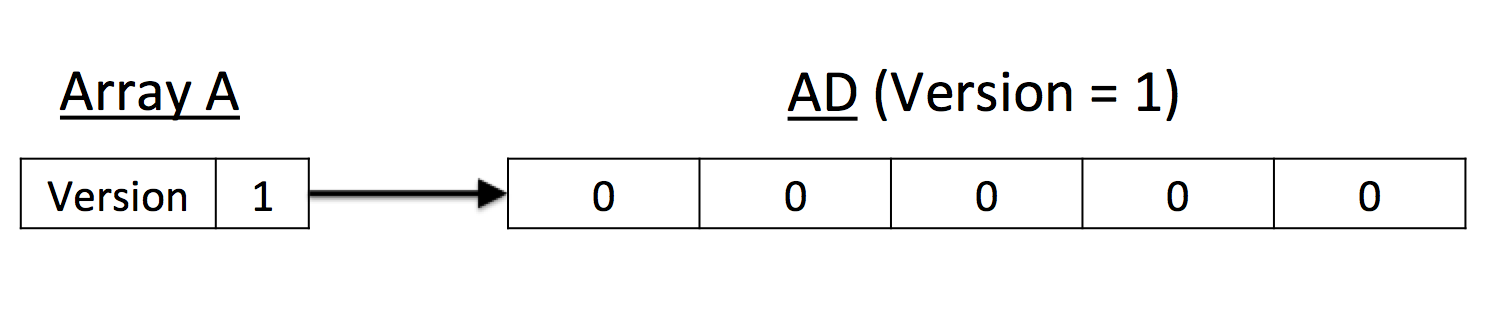
\includegraphics[scale=0.3]{new_array_A}
\nocaptionrule \caption{A = \new{}(5, 0)}
\label{fig:new_array_A}
\end{figure}

The implementation of \new{} is given below.

\begin{lstlisting}[language=ML]
val new : int ** 'a -> 'a sequence
fun new(size, init) =
  (1, (ref 1, Array.new(size, init), 
    tabulate(size, 
      fn _ => Pusharray.new$(0, \mbox{init})$)))
\end{lstlisting}

\set{} uses a compare and swap to increment the arraydata's version so that only one thread can modify an arraydata at any point in time. If the compare and swap is successful (which means the sequence is a leaf sequence), a log entry is inserted and the value array is mutated. Otherwise, the values in the sequence are copied over to produce a new arraydata. The new arraydata will have empty logs at each index. Note that the values are not directly copied into the new arraydata from the value array, we need to call \get{} at each index of the sequence when getting the values. 

The ordering of the instructions in \set{} is critical. If the vals array is modified before the log entry is inserted then a \get{} evaluated between the 2 instructions could evaluate to the wrong value.

Figure \ref{fig:set_old_array} visualizes \set{}s on interior and leaf sequences.
\begin{figure}[!ht]
\centering
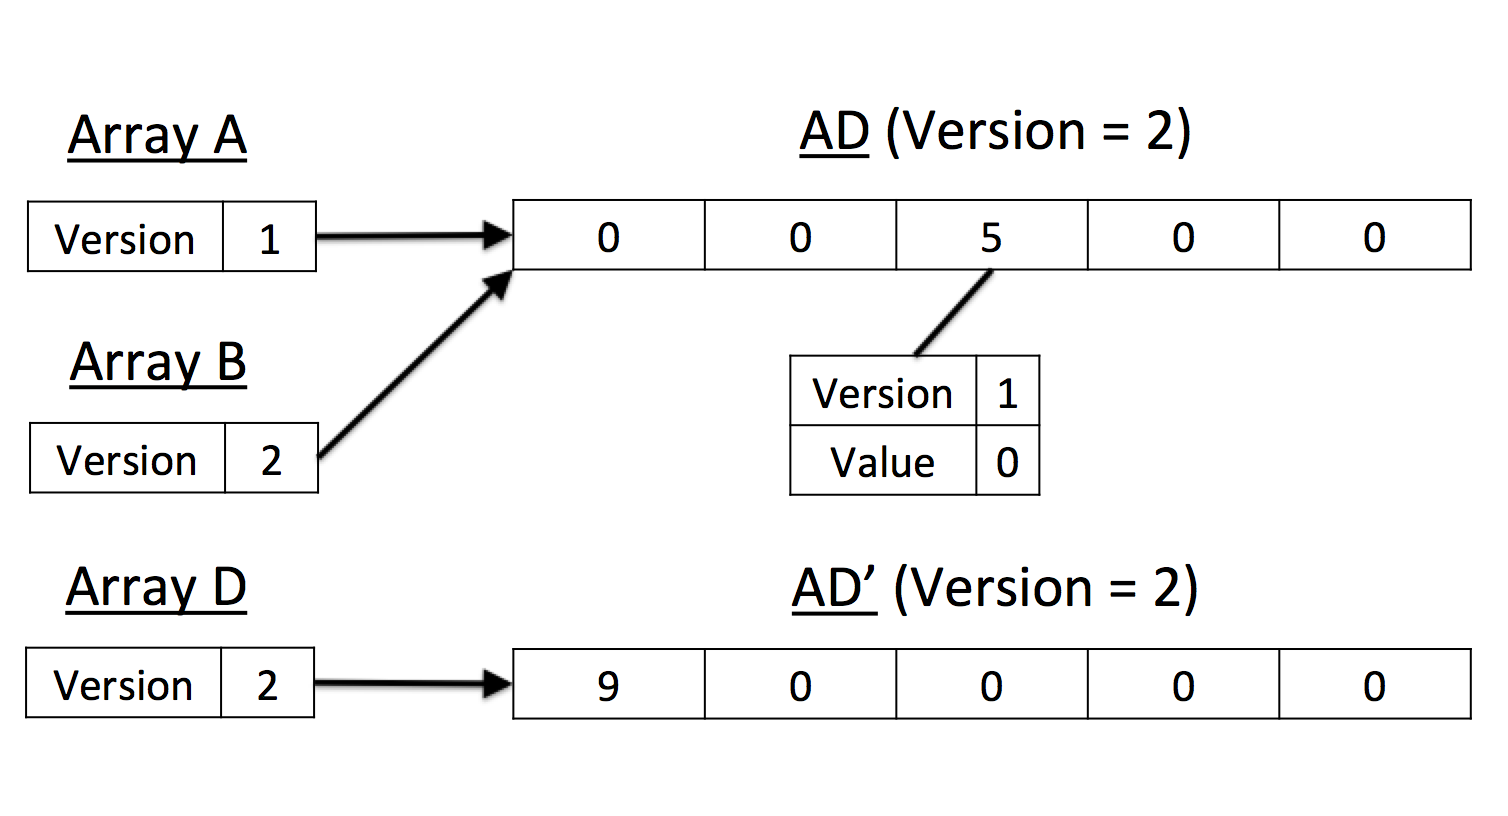
\includegraphics[scale=0.3]{set_old_array}
\nocaptionrule \caption{$B = \tset(A, 2, 5)$ changes the value array and adds a log entry. Then $D = \tset(A, 0, 9)$ creates $AD'$ because $A$ is interior.}
\label{fig:set_old_array}
\end{figure}

The implementation of \set{} is given below.

\begin{lstlisting}[language=ML,escapechar=|]
val set : 'a sequence ** int ** 'a -> 'a sequence
fun set$((V,(V_r, A, L)),i,v)$ = 
  if not(cmpswap$(V_r, V, (V+1))$)|\label{line:set-cmpswap}| orelse
     (!$V_r \bmod \mbox{length}(A) = 0$) then
    let val $A'$ = getFarrayValues$((V,(V_r, A, L)))$
       val $L'$ = emptyLogs(size($A$))
    in update$(A', i, v)$; $(1, (\mbox{ref }1, A', L')$ 
    end
  else
    Pusharray.push$(\mbox{sub}(L,i),(V,\mbox{sub}(A,i)))$; |\label{line:start-cmpswap}|
    update$(A, i, v)$;
    $(V+1, (V_r, A, L))$ |\label{line:end-cmpswap}|
\end{lstlisting}

\get{}$(A,i)$ first loads the value $v$ at the $i^{\text{th}}$ index of the value array. If the sequences' version and corresponding arraydata's version match (meaning that the sequence is a leaf sequence), then \get{} evaluates to $v$. If the log at index $i$ is empty or all versions in the log at index $i$ are less than the sequence version, then \get{} evaluates to $v$. Otherwise, \get{} binary searches the log at index $i$ for the value corresponding to the least version $\geq$ the sequence's version.

As in \set{}, the ordering of the instructions in \get{} is important. In particular, index $i$ of the value array must be loaded before the versions are compared or the logs are examined. If the versions are compared first and a \set{} is evaluated between the 2 instructions, the \set{} might modify the value array and cause the \get{} to evaluate to the wrong value.

The implementation of \get{} is given below.

\begin{lstlisting}[language=ML,escapechar=|]
val get : 'a sequence ** i -> 'a
fun get$((V, (V_r, A, L)),i)$ =
let val guess = sub$(A,i)$ |\label{line:load-value}|
   val $l$ = sub$(L, i)$
   val $n$ = Pusharray.size$(l)$
in if $V = \;!V_r$ then guess |\label{line:get-version-check}|
   else if $n = 0$ then guess |\label{line:log-empty}|
   else
      let val $(V', \_)$ = Pusharray.get$(l, n-1)$
      in if $V' < V$ then guess |\label{line:log-small}|
        else valueAtLeastVersionGeq$(l,V)$ |\label{line:binary-search}|
      end
\end{lstlisting}

\subsection{Target Language}

For our proofs we give a more formal definition of the target language in which we implement sequences\footnote{Our target language is different from the SML-like code used in the code samples. This for clarity of our code samples. It is easy to translate our code samples to our target language.}. The target language extends the source language to support mutable references and compare and swap. The structural dynamics of the target language is given by the following judgement, where $(\pi, \mu)$ is the memory and $(\pi', \mu')$ is the memory after the step has been taken,
$$(\pi, \mu), e \to_T (\pi', \mu'), e'$$

For simplicity we assume all sequences and arraydatas are int sequences and int arraydatas. To avoid dealing with overflow issues, we assume that all integers in the target language are unbounded. Sequences are represented as $\&l$ where the label $l$ indexes into the store $\pi$.

The memory contains an immutable store $\pi$ that maps labels to $(\lambda, *k)$ where $\lambda$ is an integer version number and $k$ is an index into $\mu$. Intuitively, $\pi$ contains all the sequences created so far in the evaluation of the expression. New key-value pairs can be inserted into $\pi$ but existing mappings cannot be modified. The memory also contains a mutable store $\mu$ that maps labels to values $(V, A, L)$ of type int arraydata. 

For concision we do not give the full dynamics of our target language. As examples, we give the rules for creating a new arraydata, pushing a log entry, and compare and swap. Let $a_n$ denote an array of $n$ $a$s and let $\{\}$ denote an empty $(\mbox{int} * \mbox{int})$ pusharray.
$$\frac{n \text{ int val} \;\;\; k \not\in L(\mu)}{(\pi, \mu), \mbox{\func{newad}}(n) \to_T (\pi, \mu[k \mapsto (0, 0_n, \{\}_n)]), *k}\text{ (new-ad)}$$

$$\frac{V, V' \text{ int val} \;\;\; \mu[k] = (V, A, L)}{(\pi, \mu), \mbox{\func{cmpswap}}(*k, V, V') \to_T (\pi, \mu[k \mapsto (V', A, L)]), \text{true}}\text{ (cas-true)}$$

$$\frac{V, V' \text{ int val} \;\;\; \mu[k] \neq (V, A, L)}{(\pi,\mu), \text{\func{cmpswap}}(*k, V, V') \to_T (\pi,\mu), \text{false}}\text{ (cas-false)}$$

$$\frac{\begin{gathered}\mu[k] = (V, A, L) \;\;\; i, V', v \text{ int val} \;\;\; \\ L[i] = (p_1, ..., p_n) \;\;\; L' = L[i \mapsto (p_1, ..., p_n, (V',v))]\end{gathered}}{(\pi,\mu), \text{\func{push}}(*k, i, (V', v)) \to (\pi,\mu[k \mapsto (V, A, L')]), *k} \text{ (push)}$$

In the source language, evaluating \new{}, \get{}, and \set{} involves a single step. In the target language, \new{}, \get{}, and \set{} are function calls to our implementation. Evaluating the function calls requires multiple steps. Let $C(\tnew{})$, $C(\tget{})$, $C(\tset{})$ be the implementation (that is, the lambda expression) for \new{}, \get{}, and \set{} respectively. 

The following rules show the evaluation of \get{} and \set{} in the target. \get{} is simply substituted with its implementation. For \set{}, we use a \set{}' ``wrapper" so that the sequence \set{} evaluates to can be added to the store $\pi$ in the end-set rule. We keep track of the sequences created so we can show invariants on sequences in our proof of correctness.

$$\frac{i \text{ int val}}{(\pi, \mu), \tget{}(\&l, i) \to_T (\pi, \mu), C(\tget{})(\&l, i)} \text{ (get)}$$

$$\frac{i, v \text{ int val}}{(\pi,\mu), \text{\set{}}(\&l, i, v) \to_T (\pi, \mu), \text{\set{}}'(C(\text{\set{}})(\&l, i, v))} \text{ (start-set)}$$

$$\frac{(\pi, \mu), e \to_T (\pi',\mu'), e'}{(\pi,\mu), \text{\set{}}'(e) \to_T (\pi',\mu'), \text{\set{}}'(e')} \text{ (eval-set)}$$

$$\frac{l \not\in L(\pi)}{(\pi, \mu), \text{\set{}}'((V,*k)) \to_T (\pi[l \mapsto (V, *k)], \mu), \&l} \text{ (end-set)}$$

The rules for \new{} are similar to \set{}. As in the source structural dynamics, either side of a fork-join expression in the target can take a step. This makes the target structural dynamics non-deterministic. However, because \get{} and \set{} involve multiple steps, the target has a greater number of possible interleavings than the source.

\begin{definition}
A transition sequence in the target language is a sequence of memory stores $[(\pi_0, \mu_0), ..., (\pi_n, \mu_n)]$ and expressions $[e_0, ..., e_n]$ such that for all $0 \leq i < n$, $(\pi_i, \mu_i), e_i \to_T (\pi_{i+1}, \mu_{i+1}), e_{i+1}$. We say that $(\pi_0, \mu_0), e_0 \to^*_T (\pi_n, \mu_n), e_n$ or $(\pi_0, \mu_0), e_0, \to^n_T (\pi_n, \mu_n), e_n$.
\end{definition}

An expression $e$ in the source language is compiled to an expression $e'$ in the target and then executed according to the target's dynamics. Since the source language is a subset of the target language, $e = e'$. In other words an expression $e$ in the source language can be viewed as an expression in the target.

We show that our implementation of sequences in the target correctly implements the source. The non-atomicity of \set{} and \get{} means that we cannot appeal to standard parametricity theorems for our proofs.

\subsection{Proof of Correctness}

The full correctness proof follows along the lines of~\cite{concurrent-logical} and~\cite{concurrent-logical2}. We concentrate here on the critical parts, involving \new{}, \get{}, and \set{}. We give a rely-guarantee style argument~\cite{rely-guarantee} for the correctness of our implementation (for integer sequences).

We show invariants on the memory store and constraints on the possible ways that the memory store can evolve in a valid target program. Given these invariants and constraints, we show that \new{}, \get{}, and \set{} behave the same way in the source and target. The tricky part of the proof is setting up the invariants and theorems---the proofs follow from extensive but straightforward casework.

\begin{definition}
(Valid memories) Consider memory store $(\pi, \mu)$. Consider arbitrary label $l \in L(\pi)$ and suppose $\pi[l] = (\lambda, k)$. We say $(\pi, \mu)$ is valid at $l$ if the following hold.
\begin{enumerate}
\item $k \in L(\mu)$. Assuming this is true, let $\mu[k] = (V, A, L)$.
\item $0 \leq \lambda \leq V$
\item For all $i$ and $0 \leq j < \text{\func{len}}(L[i])$ if $L[i][j] = (V', v)$ then $V' < V$
\item For all $i$ and $0 \leq j < k < \text{\func{len}}(L[i])$, if $L[i][j] = (V_1, v_1)$ and $L[i][k] = (V_2, v_2)$ then $V_1 < V_2$
\end{enumerate}
We say $(\pi, \mu)$ \emph{valid} if for all $l \in L(\pi)$, $(\pi, \mu)$ is valid at $l$. 
\end{definition}

\begin{theorem}
Let $e$ be an expression in the source language. Suppose that $(\{\}, \{\}), e \to^*_T (\pi, \mu), e'$. Then $(\pi, \mu)$ \emph{valid}.
\end{theorem}

\begin{proof}
(Outline) By induction on the length of the transition sequence taking $(\{\}, \{\}), e$ to $(\pi, \mu), e'$. For the base case, verify that each condition holds for $(\{\}, \{\})$. 

Our IH is that that the theorem holds for all transition sequences of length $n$. We then consider an arbitrary transtion sequence of length $n+1$. From the IH, the first $n$ steps leads to a valid memory state. We then case on all possible modifications that the $n+1^{\text{th}}$ step can make to memory. Showing properties (1) to (3) is straightforward. To prove property (4), we need to appeal to a lemma that different executions of lines~\ref{line:start-cmpswap} to~\ref{line:end-cmpswap} in the implementation of \set{} on the same arraydata cannot overlap. The lemma holds because of property (2) and the compare and swap.
\end{proof}

\begin{definition}
(Memory transformations) Consider $(\pi, \mu), (\pi', \mu')$ \emph{valid} \footnote{Note that the relation is only defined for valid memory states.}. Consider arbitrary label $l$ with $l \in L(\pi)$ and $l \in L(\pi')$. Suppose that $\pi[l] = (\lambda, k)$ and $\pi'[l] = (\lambda', k')$. We say that $(\pi, \mu) \leq (\pi, \mu)$ at $l$ if the following hold.
\begin{enumerate}
\item $\lambda = \lambda'$ and $k = k'$ (in other words, values in $\pi$ are immutable). Assuming this is true, let $\mu[k] = (V, A, L)$ and $\mu'[k] = (V', A', L')$.
\item $V \leq V'$. In other words, the versions are non-decreasing.
\item For all $i$, \func{len}$(L[i]) \leq$ \func{len}$(L'[i])$ and for all $i, j$ with $0 \leq j < $ \func{len}$(L[i])$, $L[i][j] = L'[i][j]$. Intuitively, this means that logs can only be extended, existing entries cannot be overwritten.
\item If \func{len}$(L[i]) <$ \func{len}$(L'[i])$ then $L'[$\func{len}$(L[i])] = (V'', A[i])$ where $V \leq V''$.
\item For all $i$, if $A[i] \neq A'[i]$ then $\lambda < V'$ and exists $0 \leq j < \text{\func{len}}(L'[i])$ with $L'[i][j] = (V'', A[i])$ and $\lambda \leq V''$.
\end{enumerate}
We say that $(\pi, \mu) \leq (\pi', \mu')$ if $L(\pi) \subseteq L(\pi')$ and for all $l$ s.t. $l \in L(\pi)$ and $l \in L(\pi')$, $(\pi, \mu) \leq (\pi', \mu')$ at $l$.
\end{definition}

\begin{lemma}
(Reflexivity) If $(\pi, \mu)$ \emph{valid} then $(\pi, \mu) \leq (\pi, \mu)$. 
\end{lemma}

\begin{lemma}
(Transitivity) If $(\pi_0, \mu_0) \leq (\pi_1, \mu_1)$ and $(\pi_1, \mu_1) \leq (\pi_2, \mu_2)$ then $(\pi_0, \mu_0) \leq (\pi_2, \mu_2)$.
\end{lemma}

\begin{theorem}
Let $e$ be an expression in the source language. Suppose that $(\{\}, \{\}), e \to^*_T (\pi, \mu), e'$ and $(\pi, \mu), e' \to^*_T (\pi', \mu'), e''$. Then $(\pi, \mu) \leq (\pi', \mu')$.
\end{theorem}

\begin{proof}
(Outline) By induction on the length of the transition sequence taking $(\pi, \mu), e'$ to $(\pi', \mu'), e''$. The base case is trivial. For the inductive step case on the possible modifications the implementation can make to memory and then use transitivity of $\leq$.
\end{proof}

\begin{definition}
Suppose $A_S, A_T$ val. We say that $\sigma, A_S \sim (\pi, \mu), A_T$ if $A_S, A_T$ have the same length and for all valid $i$, $\sigma, \tget{}(A_S, i) \to^* \sigma', v$ and $(\pi, \mu), \tget{}(A_T, i) \to^*_T (\pi', \mu'), v$ for some $v$ int val.
\end{definition}

\begin{lemma}
\label{preservation-lemma}
(Monotonicity) If $\sigma, A_S \sim (\pi, \mu), A_T$ and $(\pi, \mu) \leq (\pi', \mu')$ then $\sigma, A_S \sim (\pi', \mu'), A_T$.
\end{lemma}

Because the target language supports concurrency, the memory store might be modified (by other evaluations of \new{} and \set{}) while \new{}, \get{}, and \set{} are being evaluated. To account for this we define concurrent transition sequences.

\begin{definition}
A \emph{concurrent transition sequence} $\tau$ in the target is a left sequence of memories $[(\pi_0,\mu_0), ..., (\pi_{n-1},\mu_{n-1})]$, right sequence of memories $[(\pi_0',\mu_0'), ..., (\pi_{n-1}',\mu_{n-1}')]$ and expressions $[e_0, ..., e_n]$ with $(\pi_i,\mu_i), e_i \to_T (\pi_i',\mu_i'), e_{i+1}$ for all $i$, and $(\pi_i', \mu_i') \leq (\pi_{i+1}, \mu_{i+1})$ for all $0 \leq i < n-1$. We say that $\tau$ takes $(\pi_0, \mu_0), e_0$ to $(\pi_{n-1}',\mu_{n-1}'), e_{n-1}'$.
\end{definition}

\begin{theorem}
(\new{}) Suppose that for some $A_S, A_T$ \emph{val}, \\$\sigma, \tnew{}(n, v) \to^* \sigma', A_S$ and $(\pi, \mu), \tnew{}(n,v) \to^*_T (\pi', \mu'), A_T$. Then $\sigma', A_S \sim (\pi', \mu'), A_T$.
\end{theorem}

\begin{proof}
Because the logs are empty, \get{} on every index of $A_T$ evaluates to 0. Similarly, \get{} on every index of $A_S$ evaluates to 0.
\end{proof}

\begin{theorem}
\label{thm-get}
(\get{}) Suppose that $\sigma, A_S \sim (\pi, \mu), A_T$. Fix $i$ \emph{int val}. Suppose that $\sigma, \tget{}(A_S, i) \to^* \sigma’, v$ where $v$ \emph{int val}. Let $e_0 = \tget{}(A_T, i)$ and suppose that $(\pi, \mu) \leq (\pi_0, \mu_0)$. Consider a concurrent transition sequence from $(\pi_0, \mu_0), e_0$ to $(\pi_{n-1}', \mu_{n-1}'), e_n$ with $e_n$ \emph{int val}. Then $e_n = v$.
\end{theorem}

\begin{proof}
(Outline) We case on the line that the implementation of \get{} returns. There are 4 cases: lines \ref{line:get-version-check}, \ref{line:log-empty}, \ref{line:log-small}, and \ref{line:binary-search}. In each case, we show that $e_n$ is the same as the value $(\pi, \mu), \tget{}(A_T, i)$ evaluates to. Since $\sigma, A_S \sim (\pi, \mu), A_T$, this is the same value that $\sigma, \tget{}(A_S, i)$ evaluates to, which implies $e_n = v$.

The first case is on line \ref{line:get-version-check} in the implementation of \get{}, where \emph{guess} is returned if the version of the sequence and arraydata are the same. Since sequence versions are immutable, arraydata versions are non-decreasing, and sequence versions are $\leq$ array data versions, the sequence and arraydata versions are also the same on line \ref{line:load-value}. From the implementation of \get{}, if the entire \get{} was evaluated atomically on line \ref{line:load-value}, it would evaluate to \emph{guess}. By lemma~\ref{preservation-lemma} this means that \emph{guess} and $v$ are the same.

The other cases on lines \ref{line:log-empty} and \ref{line:log-small} are similar. In the last case, \get{} involves a binary search on the logs. The theorem follows for the binary-search case from property (3) in memory transformations (logs can only be extended) and property (4) in valid memories (versions in a log are strictly increasing).
\end{proof}

\begin{theorem}
(\set{}) Suppose that $\sigma, A_S \sim (\pi,\mu), A_T$. Fix $i, v$ \emph{int val}. Suppose that $\sigma, \tset{}(A_S, i) \to^* \sigma', A_S'$ where $A_S'$ \emph{val}. Let $e_0 = \tset{}(A_T, i, v)$ and suppose that $(\pi, \mu) \leq (\pi_0, \mu_0)$. Consider a concurrent transition sequence from $(\pi_0, \mu_0), e_0$ to $(\pi_{n-1}', \mu_{n-1}'), e_n$ with $e_n$ \emph{val}. Then $\sigma', A_S' \sim (\pi_{n-1}', \mu_{n-1}'), e_n$.
\end{theorem}

\begin{proof}
(Outline) Case on whether the compare and swap in \set{} evaluates to true or false.

If it evaluates to false, then the implementation calls \get{} at each index of $A_T$ and creates a new arraydata in $\mu$. In this case $\sigma', A_S' \sim (\pi_{n-1}', \mu_{n-1}'), e_n$ follows from theorem~\ref{thm-get}.

If it evaluates to true, then from lemma~\ref{preservation-lemma} $A_S$ and $A_T$ are related when the compare and swap evaluates. In the source, \set{}$(A_S, i, v)$ evaluates to $A_S[i \mapsto v]$. In the target, suppose that $A_T = \&l$, $\pi[l] = (\lambda, k)$ and $\mu[k] = (V, A, L)$. As argued before, different executions of lines~\ref{line:start-cmpswap} to~\ref{line:end-cmpswap} in the implementation of \set{} on the same arraydata cannot overlap. So in the target, the implementation sets $\mu[k] = (V+1,A[i \mapsto v], L')$ for some $L'$ and returns $\&l'$ s.t. $\pi[l'] = (V+1, k)$. Going through the definition of $\sim$ this gives us $\sigma', A_S' \sim (\pi_{n-1}', \mu_{n-1}'), \&l'$.

\end{proof}

\begin{theorem}
(Bounded cost) There exists $k$ s.t. if $A_T$ has size $n$ then there does not exist $(\pi, \mu)$ \emph{valid} and a concurrent transition sequence of length $> kn$ starting at either $(\pi, \mu), \tget{}(A_T, i)$ or $(\pi, \mu), \tset{}(A_T, i, v)$ for all $i, v$ \emph{int val}.
\end{theorem}

\begin{proof}
(Outline) Because we copy the contents of a sequence after $n$ updates, where $n$ is the size of the sequence, for some $k$ independent of $n$, \set{} involves at most $kn$ steps, and \get{} involves at most $k\log{n}$ steps.
\end{proof}

\subsection{Interleaved Cost Bounds}

We want to show that work done in the interleaved structural dynamics is an upper bound for the work done in the implementation. We first sketch a linearizability-type result~\cite{linearizability}.

Consider the execution $E$ of a program. We assume a sequentially consistent model of computation. Consider a sequential execution $S$ of instructions in $E$ that produces the same result as $E$. 

Consider any \get{} in the sequential execution $S$. From the previous subsection, the result that the program evaluates to does not depend on how the instructions in the \get{} are interleaved. Consider line \ref{line:get-version-check} in \get{} where the version of the array is compared with its arraydata. If the versions match then \get{} involves a constant amount of work. Otherwise, in the worst case \get{} involves a binary search on $n$ elements, where $n$ is the size of the array. This takes work proportional to $\log{n}$ \footnote{\set{} also copies the sequence data once every $n$ times the version number is increased, but the copying is amortized constant time.}.

So the execution $S$ is upper bounded (in cost) by an execution where the entire \get{} is evaluated atomically at the instruction where the versions of the array and arraydata are compared, where the \get{} has constant work if the version check succeeds and $\log{n}$ work if the check fails.

Similarly, consider any \set{} in the sequential execution $S$. From the previous subsection, the result that the program evaluates to does not depend on how the instructions in the \set{} are interleaved. Consider line \ref{line:set-cmpswap} in \set{} which involves a compare and swap on the arraydata's version. If the compare and swap is successful then \set{} involves a constant amount of work. Otherwise, in the worst case \set{} involves copying over $n$ elements, where $n$ is the size of the array. This takes work proportional to $n$.

So the execution $S$ is upper bounded (in cost) by an execution where the entire \set{} is evaluated atomically at the compare and swap instruction, where the \set{} has constant work if the compare and swap succeeds and $n$ work if the compare and swap fails.

We can trivially assume that \new{} is evaluated atomically since none of the effects of \new{} are observable until it finishes evaluating, and \new{} always takes time proportional to the size of the array being created.

We then define a relation between sequences in the source and target. $\sigma, A_S$ in the source and $(\pi, \mu), A_T$ in the target are related if \get{} evaluates to the same value at all indices, and $A_S$ is a leaf sequence if and only if $\lambda = V$ where $A_T = \&l$, $\pi[l] = (\lambda, k)$, and $\mu[k] = (V, A, L)$. We show that the relation is preserved by \new{} and \set{} and that costs of operations in the source are an upper bound for operations in the target for related sequences. Since the execution was transformed so that \new{}, \get{}, and \set{} evaluate atomically, we can then prove and apply a parametricity theorem to show that programs in the source and target evaluate to the same value.

\subsection{Parallel Cost Bounds}

Next, we sketch the case where we have an unbounded number of processors. In the worst case, \get{} involves a binary search on $n$ elements, where $n$ is the size of the array. This takes $\log{n}$ time on a machine with an unbounded number of processors. In the worst case, \set{} involves copying $n$ array elements and $n$ log entries where $n$ is the size of the array. In a machine with an unbounded number of processors, the copying can be done in $\log{n}$ time. Similarly, \new{} can execute in $\log{n}$ time on a machine with an unbounded number of processors. Note that the implementation of \new{}, \get{}, and \set{} are wait-free so these costs are independent of what other threads are doing.

It follows that we can use the evaluational dynamics to compute the work $W$ and span $S$ of evaluating an expression $e$ in our source language. We can then use theorem~\ref{thm:brent} to get that the cost of evaluating $e$ on a $p$-processor machine is $\leq c(\frac{W}{P} + S\log{P})$ for some constant $c$ independent of $e$.



\section{Test Results}
\label{sec:experiments}

Besides implementing our functional arrays in SML, we implemented our arrays in Java and compared the performance of functional arrays with regular Java arrays. Java has a relaxed memory consistency model (not a sequentially consistent memory model), so we added memory fences in suitable locations to prevent the compiler and machine from reordering instructions.

We compared the performance of leaf functional arrays and regular Java arrays of size 3,000,000 on a dual-core machine. The arrays occupied 12mb of space, and the machine had 3mb of shared L3 cache, so we ensured that the entire arrays cannot be cached. Since many of our tests involved looping and accessing elements in the array, without performing any useful computations, we disabled compiler optimizations (which optimize away the loops).

We ran each test 5 times, and took the average time. We do not show standard errors because we were interested in orders of magnitude, however all timings differed from the mean by at most $15\%$ of the mean time.

\begin{table}[h!]
\centering
\begin{tabular}{ |c|c|c|c| } 
 \hline
  & Regular & Functional & Slowdown \\ 
 \hline
 Seq. reading array & 1.35s & 1.50s & 10.8\% \\ 
 \hline
 Rand. reading array & 8.88s & 9.10s & 3.4\% \\ 
 \hline
 Seq. writing to array & 2.78s & 9.14s & 3.3$\times$ \\ 
 \hline
 Rand. writing to array & 5.57s & 13.2s & 2.4$\times$ \\ 
 \hline
\end{tabular}
\caption{Speed of leaf functional arrays vs. regular arrays in Java}
\label{mytable}
\end{table}

In the sequential read test, after creating an empty array, we sequentially get elements at indices $0,1,2,...$, starting over at $0$ when we reach the end of the array. In the random read test, we repeatedly generate a random number $r$ and get the $r^{\text{th}}$ element of the array. We performed 15,000,000 accesses in both of these tests.

In the sequential write test, starting from an empty array, we sequentially set the elements at indices $0,1,2,...$, starting over at $0$ when we reach the end of the array. In the random write test, we repeatedly generate a random number $r$ and set the $r^{\text{th}}$ element of the array. We performed 5,000,000 writes in both of these tests.

The results suggest that operations on leaf functional arrays are almost as efficient as regular arrays. The additional 2-3 times slowdown in \set{} is expected because we incur an additional cache miss when we insert a log entry. Note that similar benchmarks on alternative implementations of functional arrays, for example persistent binary search trees, are likely to be slower by a much larger factor.

Additionally, we compared the time taken to access elements in leaf arrays and interior arrays in a specific benchmark. We wrote 20,000,000 values into random indices of an array of size 2,100,000. We then read 5,000,000 values from random indices of the leaf array and the interior array. Reading from the interior array was $4.5 \times$ slower, which is not too much of a slowdown.

We also performed two simple tests to profile multi-threaded accesses in our functional array implementation. In the first test, 2 threads simultaneously accessed 500,000 random elements in an array. The total time taken was $1.77 \times$ less than a single thread accessing 1,000,000 random elements in the array. In the second test, 2 threads simultaneously accessed the same element 500,000 times. The total time taken was $1.76 \times$ less than a single thread accessing the element 1,000,000 times. The results of the second test are particularly good. We cannot expect a $2\times$ speedup because the element will keep moving between the L1 caches of the two cores. However, the speedup of $1.76 \times$ means that the accesses are not serialized (as they would be with a per-element lock).


\section{Future Work}
\label{sec:conclusion}
\begin{enumerate}
\item We do not have formal proofs for the cost bounds of our sequence implementation. Current techniques for analyzing concurrent data structures focus on proving correctness. Coming up with a framework to prove the costs of a concurrent implementation is an exciting opportunity. Note that our main results still hold without these proofs, because we present a general way to analyze data types where operating on leaf values and interior values have different costs.

\item Extending the approach of allowing operations on interior data values to be more expensive than for leaf data values to other data types (for example unordered sets or functional disjoint sets) is a possible future direction.

\item We conjecture that it is not possible for a sequence implementation to have constant (worst case) costs for all operations, which would ground the need for an implementation where costs for leaf and interior versions are different.

\item Our cost dynamics could be extended to situations that generalize beyond separate costs for interior and leaf versions. In particular, our interleaved structural dynamics does not give a tight bound for the cost of our sequence implementation. In our implementation, accessing a value in an interior version could involve constant work if there are no (or a constant number of) log entries at that index.

\end{enumerate}

% We recommend abbrvnat bibliography style.

\bibliographystyle{abbrvnat}

% The bibliography should be embedded for final submission.

\bibliography{references}

\end{document}
